\chapter{Determination of the Luminosity Correction} \label{ch:Correction}

\section{Introduction} \label{sec:corrIntro}
The goal of the luminosity measurement experiment is to find the true measure of proton-proton collisions. The LHC sends billions of protons on a head-head collision in a collection of protons called bunches, among which only some protons collide at a given time to produce secondary particles. PLT, located at about 171 cm away from the interaction point and at rapidity, $\eta$,  of $\sim$ 4, inclusively measures the charged particles. 

Within each filled bunch, the profile of the transverse density of protons is expected to be gaussian. Some protons, however, leak into neighboring bunches as seen in Figure ~\ref{fig:pBXfor}. Furthermore, protons can collide with elements within the beam pipe to produce spurious tracks. Some protons leave the ideal orbit and interact with rest gas atoms as the vacuum is not perfect, which causes secondary particle production resulting in extra tracks. 
Fig. \ref{fig:collcat} shows a schematic of tracks from several sources that can be distinguished via the track parameters--slopes, residuals. Generally, the tracks that PLT detects can be categorized as follows:


\begin{itemize}
    \item [1.] Tracks from IP   {\hfill + lumi}
    \item [2.] Tracks from IP with scatter  {\hfill + lumi}
    \item [3.] Tracks parallel to beam from collision with beam gas and obstructions far away from the IP    {\hfill - extra}
\end{itemize}




% draw collision categories
\begin{figure}[htbp!]
\centering
%\resizebox{<horizontal size>}{<vertical size>} {
%\resizebox{scale=0.8}{scale=0.8} {
	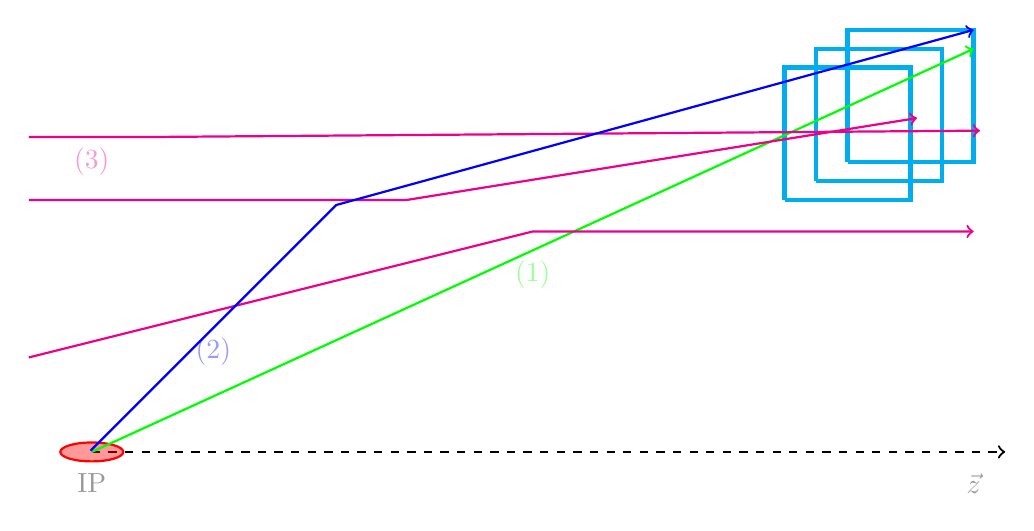
\begin{tikzpicture}[thick,fill opacity=.4,draw opacity=1,scale=0.8]
	 %three planes
	  \draw[ultra thick, cyan] (11,4) -- (13,4) -- (13,6.1) -- (11,6.1) -- (11,4);
	  \draw[ultra thick, cyan] (11.5,4.3) -- (13.5,4.3) -- (13.5,6.4) -- (11.5,6.4) -- (11.5,4.3);
	  \draw[ultra thick, cyan] (12,4.6) -- (14,4.6) -- (14,6.7) -- (12,6.7) -- (12,4.6);

	  % axes, IP
	  \draw [->, black, dashed] (0,0) --(14.5,0);
	  \node at (14,-0.5) {$\vec{z}$};
	  \draw[fill=red, red] (0,0) ellipse (0.5cm and 0.15cm);
	  \node at (0,-0.5) {IP};


	  % tracks
	  % ++ is addition to last coordinates
	  \draw [->, green] (0,0) -- node[below] {(1)} ++ (14,6.4);

	  \draw [->, magenta] (-1,5) -- node[below] {(3)} ++ (2,0) --  (14.1,5.1);
	  \draw [->, magenta] (-1,4) -- (5,4) -- (13.1,5.3);

	  \draw [->, magenta] (-1,1.5) -- (7, 3.5) -- (14,3.5);

	  \draw [->, blue] (-0.02,0.02) -- node[below] {(2)} ++ (3.9, 3.9) -- (14,6.7);

	\end{tikzpicture}
	        \captionsetup{format=hang}
	\caption{Different sources for tracks entering the PLT during proton-proton collisions. IP refers to interaction point and is the origin of genuine tracks responsible for luminosity.}
	\label{fig:collcat}
%}
\end{figure}

Two different procedures were applied for quantifying the correction term due to accidental tracks for luminosity in 2015 and 2016. Early 2015 data was compromised by the "bug" introduced during the firmware update. Algorithms used to replicate the effect in the luminosity measurement introduced by the bug will be described in section \ref{sec:firmware}, firmware issue. Procedures used to find the corrections based on track parameters for 2015 and 2016 are described in section  \ref{sec:5sigcut} and section \ref{sec:mlfit} respectively.



For the 2016 data, vdm scan data was used as a baseline to define track parameters. During vdm scan, 32 bunches are made to collide out of 3564 bunches. This means there is very small chance of the measured events to have originated from secondary collision as mentioned earlier. Section \ref{sec:mlfit} describes the theory behind the maximum likelyhood fit method used to parametrize track parameters from the vdm scan and section \ref{sec:highlumifit} provides the resulting fit to higher luminosity regime to assign a correction as a function of luminosity itself.

%move it ahead of fitting procedure?
\section{Firmware Issue} \label{sec:firmware}
%If a ROC had 3 or more hits, this would be interpreted by the FED as 0 hits which means that some of the triple coincidences were missed. The probability of getting 3 or more hits is significantly low (sub percent). To account for this issue, algorithms were written to replicate the count misses due the firmware issue using Slink data, which did not get affected by the problem. Multiple algorithms were tested, and we looked to find out the "effect" the problem had on the fast-or lumi.

%Introduced on July 31
%Fixed November 2 (between fills 4565 and fill
%4569)
%Affects a large portion of 25ns data (and the notorious fill 4246/run 254833 50ns fill)
%Two ways to measure this effect ? Transparent buffer data
%Full pixel readout (Slink)

%\subsubsection{Double Columns}

On July 31, 2015 a software bug got introduced while making a firmware update which affected how Fast-OR recognized more than 3 hits on a plane. A hit on a given plane corresponds to a charge deposit above a threshold. This charge is translated into a numerical value by the ADC in the FED. The charge deposits in every other double column are added together. Upto three levels of this signal can be distinguished to arrive at a multiplicity count inside the detector plane. The ADC value range is smaller than the dynamic range of the possible charge deposits of more than 2 hits and hence saturates. Instead of repeating the highest saturation value at high multiplicity the value was set to zero in the FED with this firmware upgrade. Hence, it reported no hit and even if the other two planes also registered at least one hit the FED would not recognize this as triple coincidence. As a result, the coincidence count underestimated by a small fraction as the likelihood for 3 hits or more on a single plane was low. To correct for this effect it was implemented algorithmically. It was decided with a counting of such cases from the ADC values obtained from a transparent buffer. 


%ADC value (which we know from gain calibration) that ought to translate to 1 coincidence count (if there was similar hit on other two planes). However, due to this bug, 3 or more hits on a single plane got translated to 0 hits. As a result, coincidence count got underestimated by a small fraction (likelihood of getting 3 hits on a plane is low) which we wanted to parametrize.

% describe what gain calibration is?

%\newcommand*{\xMin}{0}%
%\newcommand*{\xMax}{26}%
%\newcommand*{\yMin}{0}%
%\newcommand*{\yMax}{6}%
%\begin{figure}
%\centering
%\begin{tikzpicture}
%    \foreach \i in {\xMin,...,\xMax} {
%        \draw [very thin,gray] (\i,\yMin) -- (\i,\yMax)  node [below] at (\i,\yMin) {$\i$};
%    }
%    \foreach \i in {\yMin,...,\yMax} {
%        \draw [very thin,gray] (\xMin,\i) -- (\xMax,\i) node [left] at (\xMin,\i) {$\i$};
%    }
%
%\draw [step=0.5,blue, very thick] (0.25,0.25) grid (5.5,4.5);
%\draw [very thick, brown, step=0.25cm,xshift=-0.25cm, yshift=-0.25cm] (0.25,0.25) grid +(5.5,4.5);
%\end{tikzpicture}
%\end{figure}

To understand the effect of firmware issue, one has to know how FED receives signals of hits from each plane sensor. Every sensor is divided into 52 columns which is grouped into 26 double columns. Column (1,2), (3,4), (5,6) and so forth. Fast-OR records the occurrence of hits on a given double column, checks if there were hits on other two planes, and saves the result as 0/1 based on whether there was a triple-coincidence or not. The firmware undercounted the triple coincidences when one or more panels had more than 3 double columns hits for a given time period. To account for this issue, the correction was described with full pixel data. As this data contains all registered hits the expected Fast-OR rate was calculated with events that had less than 3 hits. This rate can then be compared to an accurate counts from the full pixel data to get the correction factor.

%algorithms were written to replicate the count misses due the firmware miscount using Slink data, which did not get affected by the problem. Multiple algorithms were tested, and we looked to find out the "effect" the problem had on the fast-or lumi because we don't exactly know the exact behaviour/response of detector readout under these conditions--how are pixels interpreted when adjacent columns get hit or when adjacent double columns were hit and so forth.

%Double columns
%DataHistogramsDat
%Add correction (delL/sbil) plot from transparant buffer, and algorithm replication here.
%clusters, extra clusters?

\newpage
\begin{samepage}

\begin{figure}[htbp!]
\centering
  \includegraphics[width=0.75\textwidth]%
    {figures/FastOr/firmwareRate.png}% picture filename
        \captionsetup{format=hang}
    \caption{Missing Pixel rate from Fill 4444 averaged over 5 minute interval. Missing rate from the transparant buffer is represented by $+$.}
    \label{fig:Miss_Rate}
\end{figure}

%\textcolor{red}{algo1}: count of the total number of double columns.
%
%\textcolor{green}{algo3}: count of double columns with non-adjacent columns
%
%\textcolor{yellow}{algo4}: count of double columns with non adjacent rows,columns
%
%\textcolor{blue}{algo2}: count of non-adjacent double columns


The red points(\textcolor{red}{algo1}) simply counts the number of double columns and is therefore higher than the rate from the transparent buffer. This overcounting occurs as adjacent double columns are blinded by choice of the trigger on the readout chip.
The yellow points(\textcolor{yellow}{algo4}) includes the requirement for adjacent columns on both rows and columns and is therefore lower than red and lower than the rate from the transparent buffer. This is expected as FED only checks for adjacency requirement on columns.  The green points (\textcolor{green}{algo3}) counts the number of double columns with non-adjacent columns and the blue points (\textcolor{blue}{algo2}) simply counts the number of non-adjacent double columns, both of which undershoot the rate found via the transparent buffer. This simply demonstrates that the trigger based on double columns in the readout chip does not consistently blind adjacent columns. Therefore, an average between algo1 and algo2 had to be found to match the relative rate of missing triple coincidences. This introduces some arbitrariness in the acceptance of the detector. It is included in the calibration constant $\sigma_{vis}$The rate was eventually chosen to be the one taken from the transparent buffer.

%The rate was eventually chosen to be the one taken from the transparent buffer.


%This makes sense because we know there is "some" adjacency requirement on double columns. The yellow points(\textcolor{yellow}{algo4}) checks for adjacency requirement on both rows and columns and is therefore lower than red but still lower than the rate from the transparent buffer. This also makes sense because we know there is FED only checks for adjacency requirement on columns.  The green points (\textcolor{green}{algo3}) counts the number of non-adjacent columns with non-adjacent columns and the blue points (\textcolor{blue}{algo2}) simply counts the number of non-adjacent double columns, both of which undershoot the rate found via the transparent buffer. The rate was eventually chosen to be the one taken from the transparent buffer.

\end{samepage}

%\section{Accidental Correction} \label{sec:Accidental}
%%\newpage
%Define what accidental correction means. Rename it something else?--background?

